% Chapter1.tex

\section{BP算法推导}

反向传播算法使用梯度下降策略对神经网络参数进行调整。

\subsection{全连接神经网络}

以如\reffig{fig:nn-module-complete}的三层全连接神经网络为例:

\begin{enumerate}
\item 含有$d$个神经元的输入层
\item 含有$q$个神经元的隐层
\item 含有$l$个神经元的输出层
\end{enumerate}

假设网络的激活函数都是Sigmoid函数,即$f(x)=\frac{1}{1+e^{-x}}$,每个神经元接受的输入如\reffig{fig:nn-module-complete}所示,

\begin{figure}[tbph]
\centering
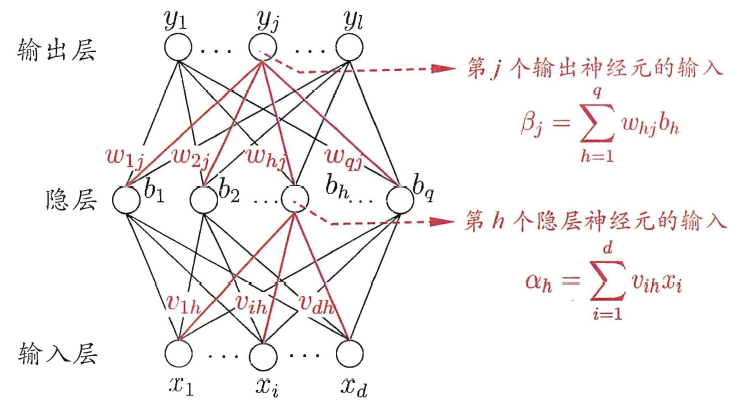
\includegraphics[width=0.75\linewidth]{.asserts/nn-module-complete}
\caption{含有单层隐含层的三层神经网络}
\label{fig:nn-module-complete}
\end{figure}

定义误差函数为$E=\frac{\sum_{i=1}^{l}{(\hat{y_i} - y_i)^2}}{2}$,即均方误差函数。以隐层到输出层的参数调整为例。

\subsubsection{权重调整}

权重$w_{ij}$的调整方式如\refeq{eq:update-w}。

\begin{equation}\label{eq:update-w}
\begin{aligned}
\Delta w_{ij} &= -\eta \frac{\partial E}{\partial w_{ij}} \\
&= -\eta \frac{\partial E}{\partial \hat{y_j}} \frac{\partial \hat{y_j}}{\partial \hat{\beta_j}} \frac{\partial \hat{\beta_j}}{\partial w_{ij}}
\end{aligned}
\end{equation}

由于$\frac{\partial E}{\partial \hat{y_j}} = \hat{y_j} - y_j$,Sigmoid函数满足$f\prime(x)=f(x)(1-f(x))$,$\frac{\partial \hat{\beta_j}}{\partial w_{ij}}=b_i$。因此\refeq{eq:update-w}可以变换为如\refeq{eq:update-w-convert}形式。

\begin{equation}\label{eq:update-w-convert}
\begin{aligned}
\Delta w_{ij} &= -\eta (\hat{y_j} - y_j) (\hat{y_j}(1-\hat{y_j})) (b_i) \\
&= -\eta b_i \hat{y_j} (\hat{y_j} - y_j) (1 - \hat{y_j})
\end{aligned}
\end{equation}

\subsubsection{阈值调整}

类似于权重调整,也对$E$求阈值$\theta$的导数。

\begin{equation}\label{eq:update-theta}
\begin{aligned}
\Delta \theta_{j} &= -\eta \frac{\partial E}{\partial \hat{y_j}} \frac{\partial \hat{y_j}}{\partial \theta_j}
\end{aligned}
\end{equation}

由于Sigmoid函数满足$f\prime(x)=f(x)(1-f(x))$,因此\refeq{eq:update-theta}可以变换为如\refeq{eq:update-theta-convert}形式。

\begin{equation}\label{eq:update-theta-convert}
\begin{aligned}
\Delta \theta_{j} &= -\eta (\hat{y_j} - y_j) (-1)(\hat{y_j}(1-\hat{y_j}))\\
&= \eta \hat{y_j} (\hat{y_j} - y_j) (1-\hat{y_j})
\end{aligned}
\end{equation}

每次训练后,朝误差减少的方向调整参数。其中$\eta$是学习率。

\subsection{卷积神经网络}

以28*28的输入图像,一层卷积、一层池化、一层全连接的神经网络为例,如\reffig{fig:cnn-example-1}。CNN的模型参数只有卷积层的权值矩阵和偏置,全连接层的权值矩阵和偏置。因此求导顺序如下:

\begin{enumerate}
\item 交叉熵损失函数
\item softmax激活函数
\item 全连接层
\item 池化层
\item sigmoid激活函数
\item 卷积层
\end{enumerate}

\subsubsection{交叉熵损失函数}

交叉熵定义为$CELF=-(\sum_{k=1}^{n}y_klog(\hat{y_k}))$,因此其导数定义如\refeq{eq:CELF}。

\begin{equation}\label{eq:CELF}
\begin{aligned}
\frac{\Delta CELF}{\Delta \hat{y_k}} &= -\frac{y_k}{\hat{y_k}}
\end{aligned}
\end{equation}

\subsubsection{softmax激活函数}

softmax激活函数定义为$y_i = \frac{e^{x_i}}{\sum_{k=1}^{n}{x_k}}$,其导函数定义如\refeq{eq:softmax-bp}。

\begin{equation}\label{eq:softmax-bp}
\begin{aligned}
\frac{\partial y_i}{\partial x_j} &=
\begin{cases}
\frac{e^{x_j}(\sum_{k=1}^{n}{e^{x_k}} - e^{x_j})}{(\sum_{k=1}^{n}{e^{x_k}})^2} = y_i(1-y_i), & \text{i == j} \\
\frac{0-e^{x_i}e^{x_j}}{(\sum_{k=1}^{n}{e^{x_k}})^2} = -y_iy_j, & \text{i != j}
\end{cases}
\end{aligned}
\end{equation}

求softmax激活函数的输入$x_i$对于CELF的导数如\refeq{eq:CELF-softmax}。

\begin{equation}\label{eq:CELF-softmax}
\begin{aligned}
\frac{\partial CELF}{\partial x_i} &= \sum_{k=1}^{n}{\frac{\partial CELF}{\partial y_k} \frac{\partial y_k}{x_i}} \\
&=  -\frac{y_i}{\hat{y_i}}\hat{y_i}(1-\hat{y_i}) + \sum_{k \neq i}\frac{y_k}{\hat{y_k}} {\hat{y_i}\hat{y_k}} \\
&= y_i\hat{y_i} + \sum_{k \neq i}{y_k\hat{y_i}} - y_i \\
&= \hat{y_i}\sum_{k=1}^{n}{y_k} - y_i \\
&= \hat{y_i} - y_i
\end{aligned}
\end{equation}

\subsubsection{全连接层}

全连接层可以由$y=\sum_{k=1}^{n}{x_k w_k} + b$,其中$w_k$是第$k$个输入$x_k$的权重。因此其对$w_k$和$b$的导数定义为如\refeq{eq:affine-bp}。

\begin{equation}\label{eq:affine-bp}
\begin{aligned}
\frac{\Delta y}{\Delta w_i} &= x_i \\
\frac{\Delta y}{\Delta b} &= 1
\end{aligned}
\end{equation}

由此得到CELF对权重$w_k$和偏置$b$的导数如\refeq{eq:CELF-affline-w-b}。其中$x_i$为softmax激活函数的输入,$w_j$为全连接层第$j$输入$a_j$的权重

\begin{equation}\label{eq:CELF-affline-w-b}
\begin{aligned}
\frac{\partial CELF}{\partial w_j} &=
\frac{\partial CELF}{\partial x_i} \frac{\partial x_i}{\partial w_j} \\
&= (\hat{y_i} - y_i)a_j \\
\frac{\partial CELF}{\partial b} &=
\frac{\partial CELF}{\partial x_i} \frac{\partial x_i}{\partial b} \\
&= (\hat{y_i} - y_i)
\end{aligned}
\end{equation}

由于下面的卷积层仍然需要用到全连接层对输入的导数,因此求出CELF对输入$a_j$的导数如\refeq{eq:affine-a-bp}。

\begin{equation}\label{eq:affine-a-bp}
\begin{aligned}
\frac{\partial CELF}{\partial a_j} &=
\frac{\partial CELF}{\partial x_i} \frac{\partial x_i}{\partial a_j} \\
&= (\hat{y_i} - y_i)w_j
\end{aligned}
\end{equation}

\subsubsection{池化层}

池化层对全连接层的输入进行了重新排列组合并加权平均。池化层的输入和输出分别是$[c_1, c_2, \dots, c_{2n^2}]$和$[a_1, a_2, \dots , a_{n^2}]$,其对应关系可以用\refeq{eq:pooling-bp}描述。

\begin{equation}\label{eq:pooling-bp}
\begin{aligned}
a_i &= \frac{ 
c_{2 [\frac{i}{n}] \times 2n + 2(i \% n)} +
c_{2 [\frac{i}{n}] \times 2n + 2(i \% n + 1)} + 
c_{2 ([\frac{i}{n}] + 1) \times 2n + 2(i \% n)} + 
c_{2 ([\frac{i}{n}] + 1) \times 2n + 2(i \% n + 1)} }
{4}
\end{aligned}
\end{equation}

池化层的导数恒为$\frac{1}{4}$,因此对于梯度下降并没有影响。

\subsubsection{sigmoid激活函数}

sigmoid激活函数定义为$c=\frac{1}{1+e^{-d}}$,sigmoid的导函数如\refeq{eq:sigmoid-bp}。

\begin{equation}\label{eq:sigmoid-bp}
\begin{aligned}
\frac{\partial c}{\partial d} = c(1-c)
\end{aligned}
\end{equation}

\subsubsection{卷积层}

卷积层对输入的图像执行了卷积操作,可以用如\refeq{eq:convolution-layer}描述卷积层执行的操作。

\begin{equation}\label{eq:convolution-layer}
\begin{aligned}
\begin{bmatrix}
d_1 \\ d_2 \\ \dots \\ d_m
\end{bmatrix}
&=
\begin{bmatrix}
u_{11} & u_{12} & \dots & u_{1n} \\
u_{21} & u_{22} & \dots & u_{2n} \\
\dots & \dots &   & \dots \\
u_{m1} & u_{m2} & \dots & u_{mn} 
\end{bmatrix}
\times
\begin{bmatrix}
v_1 \\ v_2 \\ \dots \\ v_n
\end{bmatrix}
+
\begin{bmatrix}
q \\ q \\ \dots \\ q
\end{bmatrix}
\end{aligned}
\end{equation}

因此,卷积层的导数如\refeq{eq:convolution-bp}。

\begin{equation}\label{eq:convolution-bp}
\begin{aligned}
\frac{\partial d_i}{\partial v_j} &= u_{ij} \\
\frac{\partial d_i}{\partial q} &= 1
\end{aligned}
\end{equation}

最终推出CELF对权重$v_k$和偏置$q$的导数公式如\refeq{eq:CELF-v-q},其中$\frac{\partial CELF}{\partial a_j}$是$CELF$对全连接层输入$a_j$的导数,$\frac{\partial a_j}{\partial c_l} \frac{\partial c_l}{\partial d_l}$是$a_j$对卷积层输出$d_l$的导数,$\frac{\partial d_l}{\partial v_k}$是卷积层输出$d_l$对权重$v_k$的导数。

\begin{equation}\label{eq:CELF-v-q}
\begin{aligned}
\frac{\partial CELF}{\partial v_k} &=
\sum_{j}\frac{\partial CELF}{\partial a_j} % CELF、softmax、全连接
\sum_{l}\frac{\partial a_j}{\partial c_l} \frac{\partial c_l}{\partial d_l} % 池化、sigmoid
\frac{\partial d_l}{\partial v_k} \\ % 卷积
&=
\sum_{j}(\hat{y_i} - y_i)w_j % CELF、softmax、全连接
\sum_{l}\frac{1}{4}c_l(1-c_l) % 池化、sigmoid
u_{lk} \\ % 卷积
\frac{\partial CELF}{\partial b} &=
\sum_{j}\frac{\partial CELF}{\partial a_j} % CELF、softmax、全连接
\sum_{l}\frac{\partial a_j}{\partial c_l} \frac{\partial c_l}{\partial d_l} % 池化、sigmoid
\frac{\partial d_l}{\partial b} \\ % 卷积
&=
\sum_{j}(\hat{y_i} - y_i)w_j % CELF、softmax、全连接
\sum_{l}\frac{1}{4}c_l(1-c_l) % 池化、sigmoid、卷积
\end{aligned}
\end{equation}

